\documentclass[11pt]{article}
\usepackage[left= 2.5cm, right = 2.5cm,top = 2cm, bottom = 2cm]{geometry}
\usepackage{enumerate}
\usepackage{longtable}
\usepackage{amsmath,amsfonts,amssymb}
\usepackage{setspace}
\usepackage{float}
\usepackage{tabularray}
\usepackage{multicol}
\usepackage{xcolor}
\usepackage[hidelinks]{hyperref}
\usepackage{listings}
\definecolor{codegreen}{rgb}{0,0.6,0}
\definecolor{codegray}{rgb}{0.5,0.5,0.5}
\definecolor{codepurple}{rgb}{0.58,0,0.82}
\definecolor{backcolour}{rgb}{0.95,0.95,0.92}
\lstdefinestyle{mystyle}{
    backgroundcolor=\color{backcolour},   
    commentstyle=\color{codegreen},
    keywordstyle=\color{magenta},
    numberstyle=\tiny\color{codegray},
    stringstyle=\color{codepurple},
    basicstyle=\ttfamily\footnotesize,
    breakatwhitespace=false,         
    breaklines=true,                 
    captionpos=b,                    
    keepspaces=true,                 
    numbers=left,                    
    numbersep=5pt,                  
    showspaces=false,                
    showstringspaces=false,
    showtabs=false,                  
    tabsize=2
}
\lstset{style=mystyle}
\pagenumbering{gobble}
\renewcommand{\arraystretch}{1.5}
\usepackage{mathtools}
\usepackage{longtable}
\usepackage{graphicx}
\usepackage{multirow}
\usepackage{hhline}
\usepackage[utf8]{inputenc}
\usepackage[usestackEOL]{stackengine}
\setlength{\abovedisplayskip}{0in}
\setlength{\columnsep}{3em}
\newcommand{\blue}{\color{Blue}}
\newcommand{\green}{\color{Green}}
\usepackage[inkscapeformat=png]{svg}
\newcommand{\red}{\color{Red}}
\newcommand{\black}{\color{Black}}
\newcommand{\Name}{Communities }
\title{Software Requirements Analysis\\\Name : A Social Media Platform\\ SM02}
\author{Harshit Pant \\ CS21BTECH11021 \and Satpute Aniket Tukaram \\ CS21BTECH11056 \and Mahin Bansal \\ CS21BTECH11034 \and Burra Vishal Mathews \\ CS21BTECH11010}
\date{}
\begin{document}
\maketitle
\section{Overview}
\subsection{System Overview:}
The purpose of this software application is to provide a platform where users can create communities of their choice and induldge in communities of similar interests.This product intends to be a social media platform where users can create communities of their choice with different visibilities and induldge in communities of similar interests. Users can also interact with other users through direct messaging.\\
Inorder to prevent malicious users, the platform also employs a moderation system where users can report posts and comments and moderators can moderate posts and comments in their communities.
The product also intends to employ a recommender system to recommend communities and create a user-specific feed for each user.
The product also provides a end-to-end encryption for the direct messaging system.
The product is a web application and hence is intended to be independent of any underlying operating system.



The principal actors in the system are:
\begin{itemize}
    \item Guest Users: Users which have not created an account on the platform.
    \item Registered Users: Users which have created an account on the platform.
    \item Community Admins: Users which have created a community on the platform.
    \item Community Moderators: Users which have been appointed as moderators in a community.
    \item Superuser: Users which have the highest privileges on the platform.
    \item System: The system is also an actor in the system.
\end{itemize}
\subsection{System Context:}
The system aims to provide a moderated social media platform where people with similar likings can for communities and organize themselves into groups. The system also focuses on providing a user-specific feed and a direct messaging system which is encrypted and secure and cannot be read/modified by the server. Moderation system is also in place to prevent malicious users from posting inappropriate content.
\begin{figure}[H]
    \centering
    \includegraphics[width=0.95\textwidth]{../../assets/context\_diagram.jpeg}
    \caption{System Context Diagram}
\end{figure}

\subsection{Stakeholders of Communities:}
The main stakeholders of the system are:
\begin{itemize}
    \item \textbf{Guest Users}
          \begin{itemize}
              \item Guest Users can view public communities, posts and other registered users with public profiles.
              \item Guest Users can view the Trending page.
          \end{itemize}
    \item \textbf{Registered users}
          \begin{itemize}
              \item Registered can create communities with different visibilities and can join communities.
              \item Users can create posts in communities and perform other CRUD operations. They can comment on posts.
              \item Users can upvote and downvote posts and comments.
              \item Users can report posts and comments.
              \item Users can search for communities, users and posts.
              \item Users can follow other users.
              \item Users can view their user-specific-feed and their notifications.
              \item Users can use a direct messaging system to communicate with other users
          \end{itemize}
    \item \textbf{Community moderators}
          \begin{itemize}
              \item Moderators can moderate posts and comments in their communities.
              \item Community moderators can ban users from their communities.
              \item Community moderators can issue warnings to members of their communities.
          \end{itemize}
    \item \textbf{Community admins} \begin{itemize}
              \item Community admins can add and remove moderators from their communities.
              \item Community admins can delete their communities.
              \item Community admins can revoke user-bans.
          \end{itemize}
    \item \textbf{Platform admins}/\textbf{superusers} can delete users and communities.
\end{itemize}
\subsection{Scope of this Document:}
In this document we describe architecture for our software. For the purpose of this document, we will be considering the component-connector diagrams to analyze the proposed architecture of the system.
\subsection{Definitions and Acronyms:}
\begin{itemize}
    \item \textbf{CRUD} : Create, Read, Update, Delete
    \item \textbf{API} : Application Programming Interface
    \item \textbf{BLOB} : Binary Large Object
    \item \textbf{Microservices} : A software development technique—a variant of the service-oriented architecture (SOA) architectural style that structures an application as a collection of loosely coupled services.
    \item \textbf{Metadata} : Data that provides information about other data.
    \item \textbf{HTTP} : HyperText Transfer Protocol
    \item \textbf{End-to-End Encryption} : A system of communication where only the communicating users can read the messages.
    \item \textbf{Recommender System} : A subclass of information filtering system that seeks to predict the "rating" or "preference" a user would give to an item.
    \item \textbf{Moderation System} : A system to prevent malicious users from posting inappropriate content.
    \item \textbf{Direct Messaging} : A form of communication between two people that is private and secure.
    \item \textbf{Community} : A group of people with a common interest.
    \item \textbf{Cache}: A software component that stores data so that future requests for that data can be served faster.
    \item \textbf{Guest User}: A user which has not created an account on the platform.
    \item \textbf{Registered User}: A user which has created an account on the platform.
    \item \textbf{Community Admin}: A user which has created a community on the platform.
    \item \textbf{Community Moderator}: A user which has been appointed as a moderator in a community.
    \item \textbf{Superuser}: A user which has the highest privileges on the platform.
    \item \textbf{ATAM}: Architecture Tradeoff Analysis Method
\end{itemize}

\section{ Architecture Design}

\subsection{Architecture 1: The Repository Model}

\begin{itemize}
    \item This architecture revolves around the data repository, which contains communities data, user data, conversation data, roles data for communities, posts/comments data for communities and authorization data
    \item All other components are connected to data repository through different connectors
\end{itemize}

\begin{figure}[H]
    \centering
    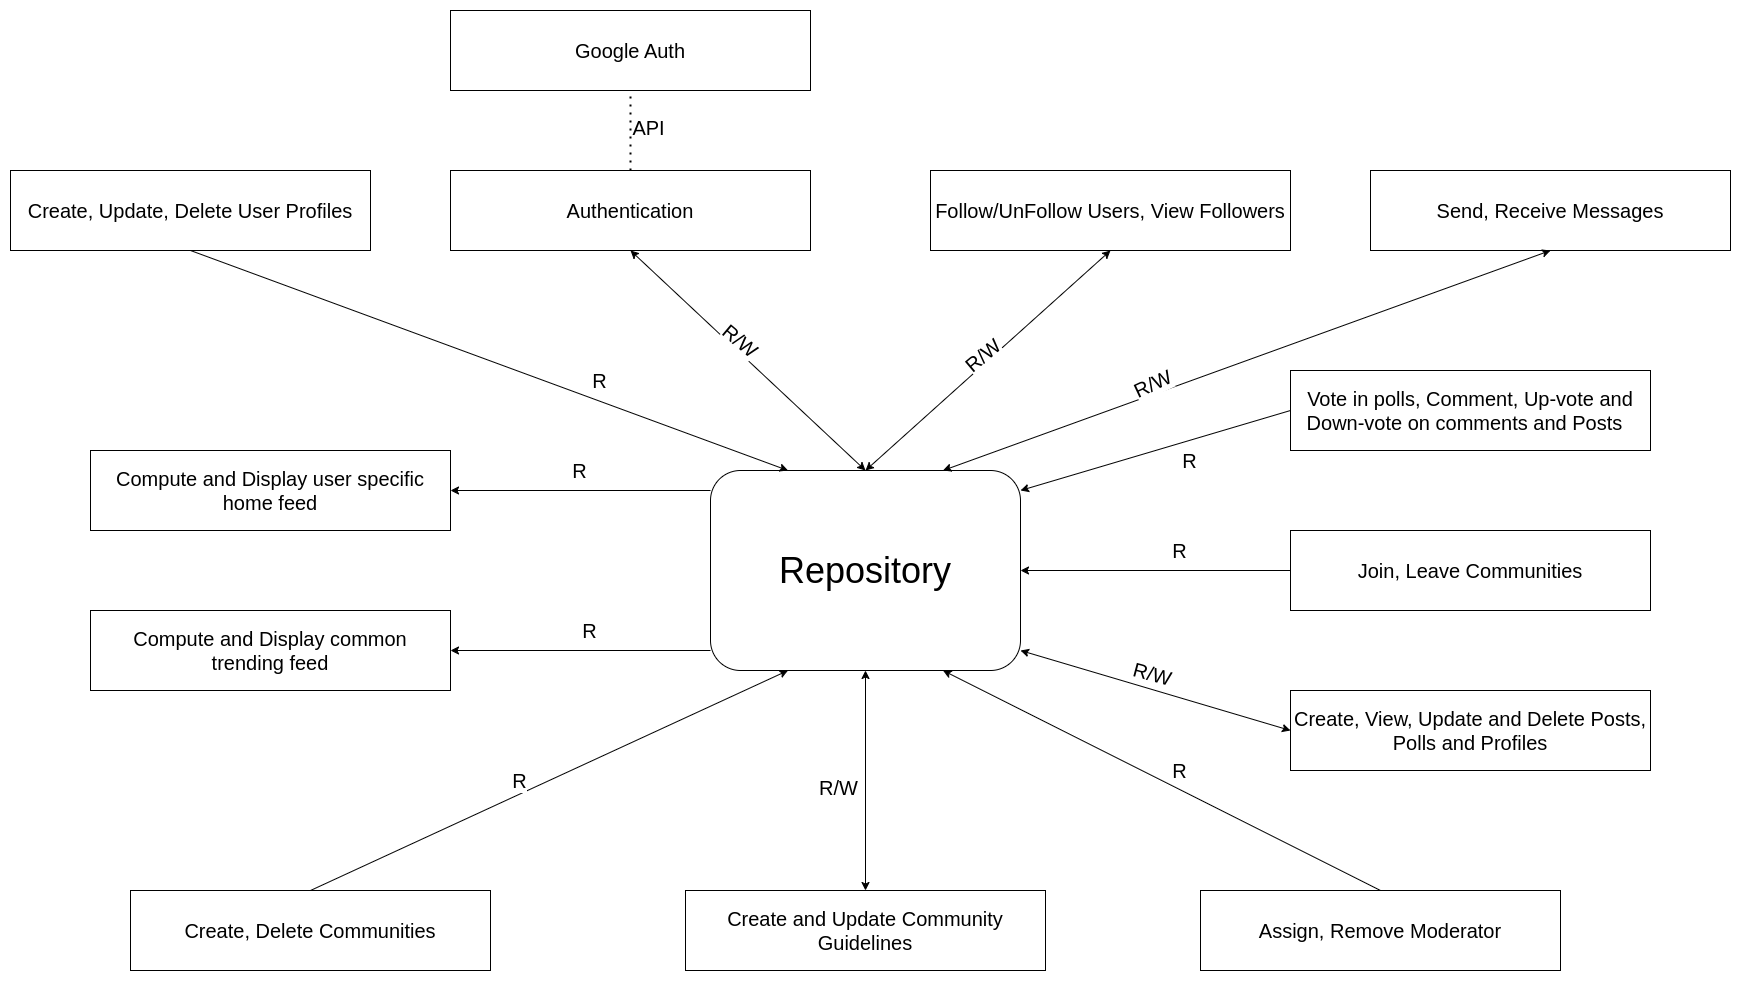
\includegraphics[width=0.95\textwidth]{../../assets/SA2.png}
    \caption{Architecture 1: The Repository Model}
\end{figure}

\SetTblrDefault{%
    stretch = 1.5,
    hlines, vlines,
    columns={c},
}
\begin{longtblr}[
    caption = {Component Description},
    label = {tab:test},
    ]{
    colspec = {|X[4]X[4]X[4]|}, % Adjusted to 3 columns
    rowhead = 1,
    hlines,
    row{even} = {gray9},
    row{1} = {olive9},
    }
    \hline
    \textbf{Component}                                                           & \textbf{Component Type}                & \textbf{Description}
    \\\hline
    \textbf{Data Repository}                                                     & Database                               & This module contains communities data, user data, conversation data, roles data for communities, post/comments data for communities, authorization data for users
    \\\hline
    \textbf{Create, Update, Delete User Profiles}                                & Database Insertion                     & This module creates, deletes and updates user profiles for which it deletes data from repository or insert different parameters in data repository
    \\\hline
    \textbf{Follow/UnFollow Users, View Followers}                               & Database Insertion and Database Access & This module allows user to view followers of other users and follow/unFollow other users in system
    \\\hline
    \textbf{Send, Receive Messages}                                              & Database Access                        & This module provides a messaging interface to users to send and receive messages from different users
    \\\hline
    \textbf{Compute and Display user specific home feed}                         & Processing(database access)            & This modules creates home feed specific to each user by using the people and communities they follows.
    \\\hline
    \textbf{Compute and Display common trending feed}                            & Processing(database access)            & This modules creates trending feed common for all users by using the recent activity in communities.
    \\\hline
    \textbf{Vote in polls, Comment, Up-vote and Down-vote on comments and Posts} & Database Access                        & This module enables user to vote in polls created by other users, Comment on different posts, up-vote or down-vote on comments  and posts created by other users
    \\\hline
    \textbf{Join, Leave Communities}                                             & Database Access                        & This module enables users to send join requests or join directly to communities and leave communities joined before
    \\\hline
    \textbf{Create, View, Update and Delete Posts, Polls and Profiles}           & Database Access                        & This module enables user too to create posts for communities, create polls, delete and update these posts
    \\\hline
    \textbf{Assign, Remove Moderator}                                            & Database Access                        & This module enables community admin to assign new moderators and remove existing moderators
    \\\hline
    \textbf{Create and Update Community Guidelines}                              & Database Access                        & This module enables community admin to create and update respective community guidelines
    \\\hline
    \textbf{Create, Delete Communities}                                          & Database Access                        & This module enables users to create communities and community admins to delete communities
    \\\hline
    \textbf{BLOB Storage}                                                        & Database                               & This module stores images and other media files
    \\\hline
    \textbf{Chat DB}                                                             & Database                               & This module stores the encrypted messages sent by users
    \\\hline
    \textbf{E2E Encryption}                                                      & Processing                             & This module encrypts and decrypts the messages sent by users
    \\\hline
    \textbf{Cache}                                                               & Database                               & This module stores frequently accessed data to improve the performance of the system
    \\\hline
    \textbf{Cache Manager}                                                       & Processing                             & This module manages the cache and updates it when the data changes
    \\\hline
    \textbf{Recommender System}                                                  & Processing                             & This module recommends communities to users based on their interests and activities
    \\\hline
    \textbf{Job Queues}                                                          & Processing                             & This module manages the background jobs such as sending notifications,managing comments, updating the cache, etc.
    \\\hline
    \textbf{API Gateway}                                                         & Processing                             & This module acts as a single entry point for all the API requests and routes the requests to the appropriate microservice
    \\\hline
    \textbf{Microservices}                                                       & Processing                             & This module contains the business logic of the application and is divided into multiple microservices such as user service, community service, post service, etc.
    \\\hline
    \textbf{Authenticaiton Service}                                              & Processing                             & This module handles the authentication of the users and generates the JWT tokens
    \\\hline
    \textbf{Cookies}                                                            & Processing                             & This module stores the session information of the users
    \\\hline
    \textbf{Scoring Service}                                                    & Processing                             & This module calculates the score of the posts and comments based on the number of upvotes, downvotes, and the time of posting
    \\\hline
    \textbf{Connections Service}                                               & Processing                             & This module manages the connections between the users such as followers, following, etc.
    \\\hline
    \textbf{Feed Service}                                                      & Processing                             & This module generates the user-specific feed and the trending feed
    \\\hline
    \textbf{Comments Service}                                                 & Processing                             & This module manages the comments trees on posts.
    \\\hline
    \textbf{Posts Service}                                                     & Processing                             & This module manages the posts and polls in the communities
    \\\hline
    \textbf{Listing Service}                                                  & Processing                             & This module manages the listing of the search results and layout of the communities and posts.
    \\\hline
    \textbf{Report Service}                                                  & Processing                             & This module manages the reporting of the posts and comments by the users
    \\\hline
    \textbf{Votes Service}                                                  & Processing                             & This module manages the voting on the posts and comments by the users
    \\\hline
    \textbf{Chat Service} & Processing & This module manages the direct messaging system
    \\\hline
\end{longtblr}

\begin{longtblr}[
    caption = {Connector Description},
    label = {tab:test},
    ]{
    colspec = {|X[4]X[4]X[4]|}, % Adjusted to 3 columns
    rowhead = 1,
    hlines,
    row{even} = {gray9},
    row{1} = {olive9},
    }
    \hline
    \textbf{Connector} & \textbf{Component Type}          & \textbf{Description}
    \\\hline
    \textbf{R}         & Database Access                  & Only reading the the data from repository
    \\\hline
    \textbf{R/W}       & Database Access and Modification & Both reading and writing data from repository
    \\\hline
    \textbf{API}       & HTTP                             & External authentication through google api and communication protocol
    \\\hline
    \textbf{Pipe}      & Pipeline                         & Data flow from one component to another                               \\\hline
    \textbf{Control}   & RPC                              & Calling a function on the server                                      \\\hline
\end{longtblr}
\subsection{Architecture 2: Layered Architecture}\\\pagebreak
\begin{figure}[H]
    \centering
    \includegraphics[width=0.95\textwidth]{../../assets/SA\_Layered.png}
    \caption{Architecture 2: Layered Architecture}

\end{figure}
\section{ATAM : Architecture Tradeoff Analysis Method}
\textbf{Here are the reasons why a layered architecture would be more suitable than a repository architecture for a this application:}

\begin{itemize}
    \item \textbf{Clear Separation of Concerns:}\\
          This application involves multiple functionalities such as user interactions, content presentation, and data storage. Layered architecture provides a clear separation of these concerns into distinct layers, making the system easier to understand and maintain.
    \item \textbf{Scalability of User Interactions:}\\
          In this app, the user interaction layer is likely to experience varying levels of demand, such as spikes in posting, commenting, or voting activities. Layered architecture allows for the independent scaling of individual layers. Thus, if there's a surge in user interactions, the corresponding layer can be scaled horizontally without impacting other layers.
    \item \textbf{Flexibility for Future Changes:}\\
          This platform may evolve over time, introducing new features or altering existing ones. Layered architecture facilitates this evolution by allowing changes to one layer without affecting others. For example, if there's a need to revamp the user interface or introduce new functionalities, modifications can be made to the respective layer without disrupting the entire system. Also the microservices layer in the architecture can be used to add new functionalities without affecting the existing ones.
    \item \textbf{Simplicity in Managing User Interactions:}\\
          This applications primarily revolve around managing user interactions, such as posting, commenting, and voting. Layered architecture simplifies the management of these interactions by providing dedicated layers for handling user input, processing business logic, and presenting data. This clarity in design aids in efficient development and maintenance of the application.
    \item \textbf{Performance:}\\
          The cache layer at the top of the data layer can be used to store frequently accessed data, which can improve the performance of the system. This can be used to store user-specific feeds and trending feeds.
    \item \textbf{Security:}\\
          The E2E encryption component can be placed in the messaging layer to ensure that the messages are secure and cannot be read by the server.
    \item \textbf{Scalability:}\\
          The layered architecture can be easily scaled horizontally by adding more instances of the same layer. This can be useful in case of a surge in user interactions or data storage requirements.
    \item \textbf{Latency}:\\
          The layered architecture can be a little slower than the repository architecture as there are multiple layers involved in processing the request. However, the layered architecture can be optimized to reduce latency by using caching and load balancing.
    \item \textbf{Debugging}:\\
          A layered architecture can be easier to debug as the concerns are separated into distinct layers. This can help in identifying the source of issues and fixing them quickly.
\end{itemize}
Hence a layered architecture is preferred for this application due to its ability to provide clear separation of concerns, scalability for user interactions, flexibility for future changes, adherence to common web application patterns, and simplicity in managing user interactions.

Below is a table comparing the two architectures based on the above points:

\begin{longtblr}[
    caption = {ATAM Analysis},
    label = {tab:test},
    ]{
    colspec = {|X[4]X[4]X[4]|}, % Adjusted to 3 columns
    rowhead = 1,
    hlines,
    row{even} = {gray9},
    row{1} = {olive9},
    }
    \hline
    \textbf{Criteria}          & \textbf{Repository Model}                                            & \textbf{Layered Model}
    \\\hline
    Data Security              & Less secure due to direct access from all modules to data            & More secure as the data access only happens through data access layer
    \\\hline
    Performance                 & Less                                                                 & More due to caching
    \\\hline
    Error Handling             & Will have to do lot of work to handle errors for different modules   & Layer wise error handling will be more efficient
    \\\hline
    Adding Features            & Difficult                                                                 & Easy as we can add an additional microservice
    \\\hline
    Code Generation Process    & Difficult as have to handle different modules completely as seperate & Easier to  work layer wise
    \\\hline
    Simultaneous user activity & Difficult to handle and Discrepancy may arrive                       & Can be done by using buffering and cache service
    \\\hline
    Database access            & Simultaneous Database access and modifications                       & Less database access due to cache service
    \\\hline
\end{longtblr}

\end{document}